\subsection{RFID}
\label{subsec:RFID}

Eine vorgesehene Funktion der Maschine ist, dass der User ohne Suchen sein Lieblingsgetränk zubereiten lassen kann. Dafür wird auf ein System zurückgegriffen, was öfters für Zutrittskontrollen oder Ähnliches verwendet wird. Nämlich RFID \footnote{Radio Frequency IDentification}.

Um schnell ein funktionierendes Teilsystem testen zu können, soll ein Breakout-Board verwendet werden. Eine Recherche hat ergeben, dass es nicht allzu viele Produkte gibt. Ein Eingenzungskriterium war, dass es es für den Ausgewählten IC eine bestehende Library gibt, welche mit Arduino oder besser C kompatibel ist. Der Chip, welcher diese Anforderungen erfüllt, ist der \textbf{Mifare MFRC522}. Dieses Brakeout-Board kann ausserdem an der Verschalung der Maschine angeschraubt werden. Somit kann er sich an einer Stelle befinden, welche weiter weg von der Hauptsplatine ist.
Das Modul arbeitet auf 13.56MHz und gilt somit als kurzwelliges System (HF).

Der MFRC522 ist der Reader im RFID-System. Er kann Daten lesen und ggf. auch schreiben. Er erzeugt ein hochfrequentes, elektromagnetisches Wechselsignal mit einer Frequenz von 13.56MHz. Der RFID-Tag wird von der Energie des Wechselsignals gespiesen. Durch Kurzschliessen der Tag-Antenne wird ein Teil der Energie des vom Reader ausgehenden Wechselfeldes verbraucht. Diese Energiedifferenz kann ein Reader detektieren. Die Reichweite für ein solches System beträgt weniger als 10cm.

Alternativ könnte ein Tag mit einer Batterie gespiesen werden. Somit erhöht sich die Reichweite des Readers, die Latenzzeiten werden kürzer und der Anwendungsbereich würde grösser.

%\begin{figure}[!h]
%\center
%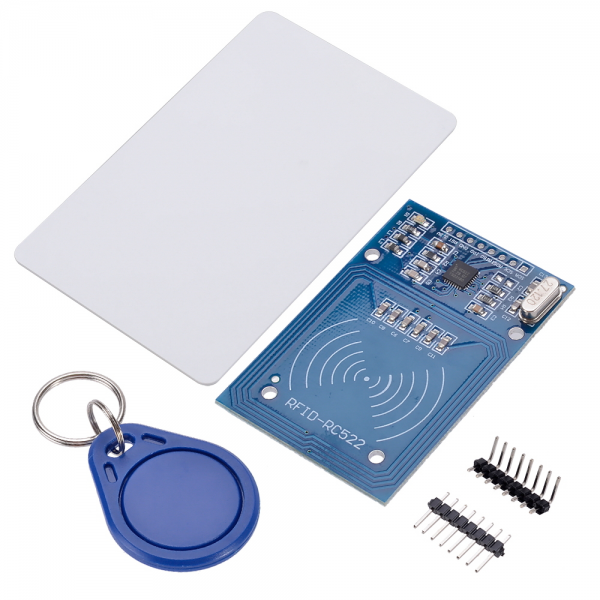
\includegraphics[width = 0.6\textwidth]{graphics/Produktbild_RFID_MFRC522}
%\caption{MFRC522.}
%\label{fig:Produktbild_RFID_MFRC522}
%\end{figure}

